\chapter{Comparison with RSiena: the same estimator, and where the speed comes from}
\label{app:samest}\label{ch:benchmark}

\graphicspath{{bench/}}

\nwsaom{} fits stochastic actor-oriented models faster than RSiena, a median factor
of \benchspmed{} over \benchnmodels{} models on one thread. A faster program may be
suspected of doing less: running fewer simulations, stopping the estimation earlier,
or approximating. This appendix sets out what was measured to rule that out. It
answers four questions: whether both programs run the same algorithm, whether they
simulate the same model, whether they give the same answers, and where the
difference in time comes from.

Every number below comes from a script in the replication package of the Stata
Journal article on \nwsaom{}; the script is named next to the number and can be
rerun. The runs were made with \nwsaom{} 1.5.7 in Stata \benchstata{} and RSiena
\benchrsiena{} in R \benchrver{}, on an \benchmachine{}, on 8 and 9 November
2026. Timings depend on the machine; the ratios between the two programs are more
stable than the seconds.

\section{The same algorithm}\label{sec:samest-alg}

Both programs estimate by the method of moments with the three-phase Robbins--Monro
algorithm of Snijders (2001), and \nwsaom{} takes RSiena's defaults. The settings
were checked against the source of RSiena \benchrsiena{} (the functions
\texttt{AnnouncePhase}, \texttt{proc2subphase}, \texttt{doIterations} and
\texttt{CalculateDerivative} of its R code); in \nwsaom{} they are in the Mata source
of the estimator. Here $p$ is the number of estimated parameters.

{\small
\begin{longtable}{@{}p{3.1cm}p{5.6cm}p{5.0cm}@{}}
\toprule
setting & \nwsaom{} & RSiena \\
\midrule
\endhead
method & method of moments & method of moments (\texttt{maxlike = FALSE}) \\
rates, one network & conditional estimation; unconditional with \opt{unconditional}, with composition change and in co-evolution models & conditional (\texttt{cond = NA}, the default); unconditional in the same cases \\
Phase 1 & $\max(50, 7+3p)$ simulations; derivatives by the score-function estimator, by finite differences if a derivative is not positive & the same \\
Phase 2 & 4 subphases, first gain 0.2, halved in each subphase; each step with the Dolby correction estimated in Phase 1 & 4 subphases, \texttt{firstg = 0.2}, \texttt{reduceg = 0.5}, \texttt{dolby = TRUE} \\
length of a subphase & at least $\lfloor 2.52\max(5, 7+p)\rfloor$ iterations, multiplied by 2.52 in each further subphase, at most that plus 200; ends early once the minimum is reached and the largest autocorrelation of the deviations is negative; stopped after 50 iterations and repeated, up to four times, if an autocorrelation falls below $-0.8$ & the same rule (\texttt{maxrepeatsubphase}) \\
Phase 3 & 1,000 simulations (\opt{k3()}) & 1,000 simulations (\texttt{n3}) \\
ministeps & one actor chosen in proportion to the rates, one tie change (or no change) chosen by the multinomial logit of the objective function; behavior: a step up, down or none & the same \\
convergence & all $t$-ratios below 0.1 and the overall maximum convergence ratio below 0.25 & the same \\
\bottomrule
\end{longtable}
}

\paragraph{What is computed differently.} Some quantities are computed in a
different way from RSiena without changing what is estimated. The linear shape
statistic of a behavior is the sum of the raw values in \nwsaom{} and of the values
centred at the overall mean in RSiena; the two differ by a constant, which cancels
in the deviations of the simulated from the observed statistics. (The quadratic
shape statistic, where centring does matter, is centred as in RSiena.) The change
statistics of a ministep are computed effect by effect over all alternatives of the
acting actor at once rather than alternative by alternative (Section~\ref{sec:samest-sim}
below); the values are the same. The random numbers differ: each simulation draws
from its own stream, derived from the seed and the position of the simulation in
the algorithm, so the estimates of the two programs, or of \nwsaom{}'s Mata engine
and its plugin, are not equal digit for digit, but they are identical in \nwsaom{}
for every number of threads. The conventions in which RSiena's definitions are
reproduced on purpose are listed in Appendix~\ref{app:quirks}.

\paragraph{Comparing the traces.} With \texttt{global NWSAOM\_TRACE 1} before the
command, \nwsaom{} prints the length of Phase 1 and the diagonal of the derivative
matrix, every 25th iteration of each Phase 2 subphase with the current parameters,
and the length of every repeated subphase. RSiena writes the same information to
its output file (the \texttt{projname} of \texttt{sienaAlgorithmCreate()}): the
Phase 1 derivatives, the iterations of each subphase and the Phase 3 summary. The
two traces can be compared line by line; they agree in the lengths of Phases 1 and
3 and in the rules that end a subphase, and differ in the Phase 2 counts only by
simulation noise (Section~\ref{sec:samest-work}).

\section{The same simulation}\label{sec:samest-fixed}

If both programs simulate the same model, they must reproduce the same statistics
at the same parameters. \texttt{R/15\_fixed\_sim.R} estimates models N1, N2 and R1
of the benchmark with RSiena (seed 1); then both programs simulate each model 1,000
times at these estimates, five times with seeds 1 to 5, without estimating
(RSiena: \texttt{simOnly = TRUE}; \nwsaom{}: \opt{theta0()} with \opt{fix(\_all)},
\texttt{stata/15\_fixed\_sim.do}). For every statistic the table gives the
$t$-ratio of the deviations from the observed value, as a mean over the five runs.
If the two programs simulate the same model, the two columns differ only by
sampling error, with a standard deviation of about $\sqrt{2/5000}=0.02$.

\begin{center}
\small
\begin{tabular}{llrr}
\toprule
model & statistic (RSiena name) & RSiena & \nwsaom{} \\
\midrule
N1 & \texttt{density} & $-0.043$ & $-0.032$ \\
 & \texttt{recip} & $-0.035$ & $-0.013$ \\
\addlinespace
N2 & \texttt{density} & $-0.003$ & $-0.016$ \\
 & \texttt{recip} & $0.006$ & $-0.003$ \\
 & \texttt{gwespFF} & $0.017$ & $0.007$ \\
\addlinespace
R1 & \texttt{density} & $0.044$ & $0.006$ \\
 & \texttt{recip} & $0.043$ & $0.013$ \\
 & \texttt{gwespFF} & $0.037$ & $-0.002$ \\
 & \texttt{transRecTrip} & $0.038$ & $0.006$ \\
 & \texttt{inPopSqrt} & $0.039$ & $-0.004$ \\
 & \texttt{outPopSqrt} & $0.045$ & $0.004$ \\
 & \texttt{sameX} & $0.068$ & $0.009$ \\
 & \texttt{egoX} & $-0.029$ & $0.013$ \\
 & \texttt{altX} & $-0.014$ & $0.031$ \\
 & \texttt{simX} & $-0.030$ & $-0.045$ \\
\bottomrule
\end{tabular}
\end{center}

All $t$-ratios are close to zero in both programs, as they must be at estimates
that satisfy the moment equations, and the two columns differ by at most 0.06, within
three standard deviations of the sampling error. RSiena's estimates are reproduced
by \nwsaom{}'s simulation, including those of the effects that \nwsaom{} computes
by a different route (Section~\ref{sec:samest-sim}).

\section{The same answers}\label{sec:samest-answers}

\nwsaom{} and RSiena were run on \benchnmodels{} models with each program's default
settings. The data of the first \benchnmain{} models are the 50-actor Glasgow panel
(RSiena's \texttt{s50}); the larger networks are 2, 4 or 10 disconnected copies of
it ($n=100$, 200, 500). Network-only models use conditional estimation, except N7
(unconditional). Models R1--R5 are applied-analysis specifications: R1 combines
\texttt{outdegree}, \texttt{reciprocity}, \texttt{gwesp()}, transitive reciprocated
triplets, square-root indegree and outdegree popularity, \texttt{samex(smoke1)} and
\texttt{egox()}, \texttt{altx()}, \texttt{simx()} on alcohol use; R2 adds alcohol as
co-evolving behavior; R3 is undirected; R4 and R5 repeat R1 and R2 on 200 actors.
The \benchnextra{} further models cover two-mode networks (X1, X2), several
networks with and without a behavior and with a non-directed network (X3--X6), and
newer single-network effects (X7). Each model was fitted with seeds 1--7 in
both programs (seeds 1--5 for fits above one minute, 1--3 for fits above three
minutes), on one thread (\texttt{stata/07\_bench\_one.do},
\texttt{R/07\_bench\_one.R}; the tables are built from one row per fit by
\texttt{tools/build\_tables.py}).

{\footnotesize
\begin{longtable}{l>{\raggedright\arraybackslash}p{0.26\textwidth}rrrrrr}
\caption{\texttt{nwsaom} and RSiena 1.6.14 on the same models and data, both single-threaded: largest difference in a mean estimate (in RSiena standard errors) and median seconds per fit}\label{tab:bench}\\
\toprule
 & Specification & $n$ & Waves & Max diff & \texttt{nwsaom} & RSiena & Speed-up \\
\midrule
\endfirsthead
\multicolumn{8}{l}{\textit{Table \thetable{} continued}}\\
\toprule
 & Specification & $n$ & Waves & Max diff & \texttt{nwsaom} & RSiena & Speed-up \\
\midrule
\endhead
\midrule
\multicolumn{8}{r}{\textit{continued on the next page}}\\
\endfoot
\bottomrule
\endlastfoot
\multicolumn{8}{l}{\textit{Network}} \\
N1 & \texttt{outdegree}, \texttt{reciprocity} & 50 & 2 & 0.06 & 0.22 & 0.84 & 3.8 \\
N2 & + \texttt{gwesp} & 50 & 3 & 0.02 & 0.52 & 1.81 & 3.5 \\
N4 & + \texttt{gwesp}, \texttt{samex()} & 50 & 3 & 0.04 & 0.60 & 2.24 & 3.8 \\
N5 & + \texttt{gwesp}, \texttt{indegpopularity}, \texttt{outactivity} & 50 & 3 & 0.08 & 0.77 & 3.02 & 3.9 \\
N6 & + \texttt{gwesp}, \texttt{egox()}, \texttt{altx()}, \texttt{simx()} & 50 & 3 & 0.04 & 0.82 & 3.57 & 4.3 \\
N7 & N2, unconditional estimation & 50 & 3 & 0.02 & 0.63 & 2.48 & 3.9 \\
\addlinespace
\multicolumn{8}{l}{\textit{Undirected}} \\
U1 & \texttt{outdegree}, default model (forcing) & 50 & 2 & 0.02 & 0.09 & 0.33 & 3.5 \\
U2 & \texttt{outdegree}, \texttt{symtype(joint)} & 50 & 2 & 0.06 & 0.09 & 1.03 & 11.5 \\
\addlinespace
\multicolumn{8}{l}{\textit{Co-evolution}} \\
C1 & N2 + alcohol: \texttt{linear}, \texttt{quadratic}, \texttt{avalt} & 50 & 3 & 0.03 & 0.98 & 4.66 & 4.7 \\
C2 & N2 + smoking: \texttt{linear}, \texttt{quadratic}, \texttt{avsim} & 50 & 3 & 0.04 & 1.05 & 5.52 & 5.2 \\
C3 & N1 + alcohol: \texttt{linear}, \texttt{avalt} & 50 & 2 & 0.03 & 0.45 & 1.84 & 4.1 \\
\addlinespace
\multicolumn{8}{l}{\textit{Realistic}} \\
R1 & full network model (see text) & 50 & 3 & 0.06 & 1.33 & 5.29 & 4.0 \\
R2 & R1 network part + alcohol co-evolution & 50 & 3 & 0.03 & 1.64 & 7.35 & 4.5 \\
R3 & undirected: \texttt{gwesp}, \texttt{samex()}, \texttt{simx()} & 50 & 2 & 0.01 & 0.24 & 0.74 & 3.1 \\
R4 & R1 & 200 & 3 & 0.06 & 22.2 & 90.1 & 4.1 \\
R5 & R2 & 200 & 3 & 0.05 & 23.6 & 109 & 4.6 \\
\addlinespace
\multicolumn{8}{l}{\textit{Larger networks}} \\
S100 & N2 & 100 & 3 & 0.05 & 1.97 & 6.82 & 3.5 \\
S200 & N2 & 200 & 3 & 0.02 & 8.30 & 31.9 & 3.8 \\
S500 & N2 & 500 & 3 & 0.03 & 64.5 & 231 & 3.6 \\
T200 & C1 & 200 & 3 & 0.08 & 13.8 & 66.5 & 4.8 \\
\addlinespace
\multicolumn{8}{l}{\textit{Two-mode}} \\
X1 & \texttt{outdegree}, \texttt{indegpopularity}, \texttt{cycle4} & 40$\times$20 & 3 & 0.10 & 0.85 & 2.75 & 3.3 \\
X2 & \texttt{outdegree}, \texttt{indegpopularity}, \texttt{outactivity}, \texttt{cycle4}, \texttt{outiso}, \texttt{antiiniso2} & 40$\times$30 & 3 & 0.03 & 0.25 & 0.61 & 2.4 \\
\addlinespace
\multicolumn{8}{l}{\textit{Two networks}} \\
X3 & both: \texttt{outdegree}, \texttt{reciprocity}; \texttt{crprod} & 50 & 3 & 0.07 & 1.41 & 3.75 & 2.7 \\
X4 & X3 without \texttt{crprod} + smoking: \texttt{linear}, \texttt{quadratic}, \texttt{avalt} (both networks) & 50 & 3 & 0.03 & 1.17 & 8.32 & 7.1 \\
X5 & X4 with \texttt{avalt} on network 1 only; \texttt{behegox}, \texttt{behaltx}, \texttt{behsim}, \texttt{samewwclosure:behavior} & 50 & 3 & 0.06 & 3.91 & 11.5 & 2.9 \\
X6 & undirected network 1 (\texttt{sym1}) + directed network 2; \texttt{crprod} & 50 & 3 & 0.03 & 1.00 & 3.08 & 3.1 \\
\addlinespace
\multicolumn{8}{l}{\textit{Single network}} \\
X7 & \texttt{outdegree}, \texttt{reciprocity}, \texttt{gwesp}, \texttt{samextranstrip()}, \texttt{altxoutact()}, \texttt{egoplusaltsqx()} & 50 & 3 & 0.02 & 2.22 & 4.26 & 1.9 \\
X8 & \texttt{outdegree}, \texttt{reciprocity}, \texttt{ownx(transtrip1 transrectrip2)} & 50 & 3 & 0.04 & 1.16 & 2.06 & 1.8 \\
\end{longtable}
}
{\par\smallskip\footnotesize Medians over seven fits (seeds 1--7; five above one minute, three above three minutes) per program (RSiena 1.6.14: 8 November 2026, X8 9 November; \texttt{nwsaom} 1.5.7: 9 November 2026; same seeds). Max diff includes the rate parameters and uses the fits that converged (overall convergence ratio $<0.25$) in both programs. N7, X1, X2: unconditional estimation in both programs (\texttt{unconditional}; \texttt{cond = FALSE}); X3--X6: \texttt{nwsaom multinet} with \texttt{k0(100) k3(1000)} against RSiena \texttt{n3 = 1000, nsub = 4}. Fits that converged, RSiena / \texttt{nwsaom}, for the models with at least one that did not: C2 6/6, 6/7; R2 6/7, 7/7; R4 4/5, 7/7; R5 4/5, 6/7; X1 1/7, 7/7; X3 7/7, 5/7; X4 6/7, 6/7; X5 6/7, 7/7.\par}


Over all \benchnparams{} parameters the mean estimates over seeds differ by at most
\benchmaxdiff{} RSiena standard errors (on average \benchmeandiff{}), which is the
size of RSiena's own variation between seeds (median \benchseedsd{} standard errors,
at most \benchseedsdmax{}). The standard errors, themselves simulation estimates, agree (as medians
over seeds) within \benchnetsepct\% for the network models; over all models the
ratio of the two programs' standard errors is between \benchserlo{} and
\benchserhi{}.

Of the \benchfits{} \nwsaom{} fits, \benchnwconv{} converged by RSiena's criterion
(overall maximum convergence ratio below 0.25), and \benchrsconv{} of RSiena's
\benchrsfits{}. Fits that did not converge are not used in the comparison of the
estimates. \nwsaom{} converged less often than RSiena only in X3 (5 of 7 fits
against 7 of 7). This is chance: with seeds 1 to 20 the overall maximum
convergence ratio of X3 had a median of 0.12 in \nwsaom{} and 0.14 in RSiena, and it
was above 0.25 for two seeds in \nwsaom{} (3 and 6, the two of the benchmark) and
for one in RSiena; the estimates of the two fits that did not converge agree with
RSiena's as well.

\begin{figure}[htbp]
\centering
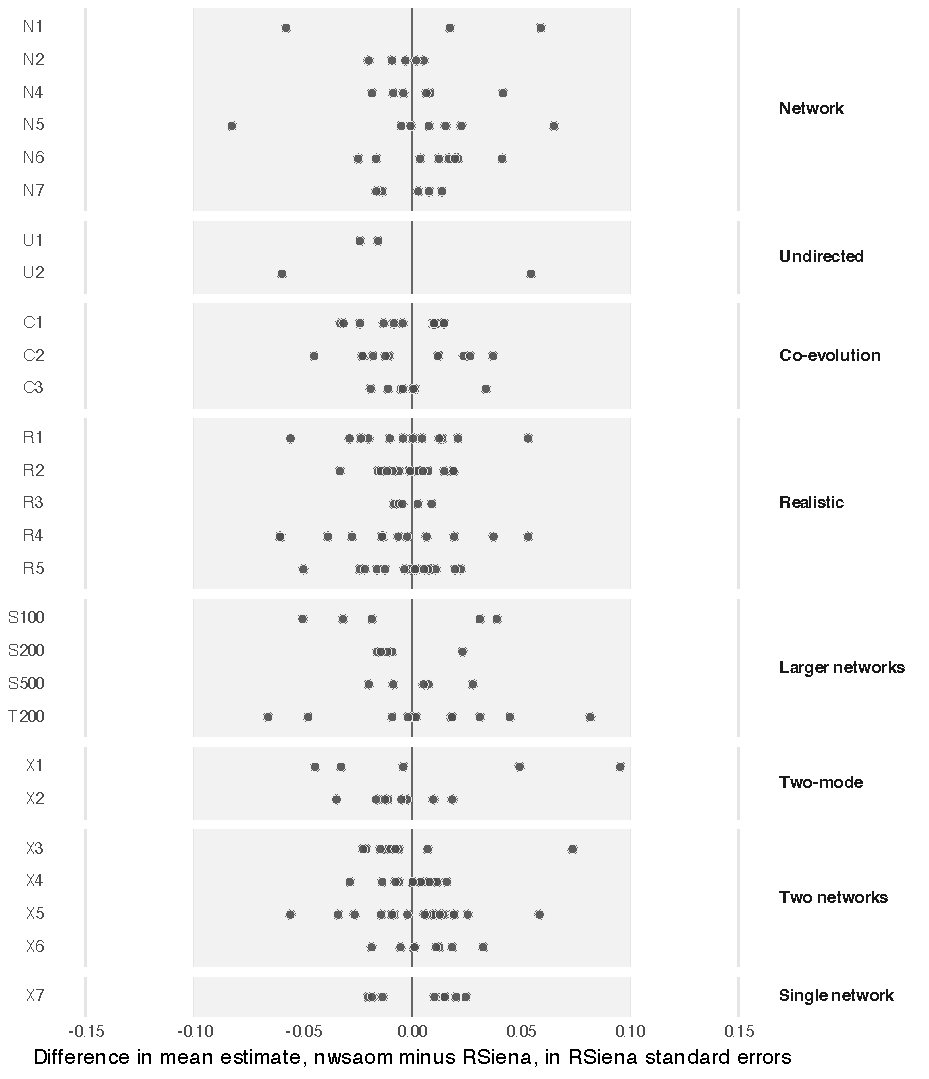
\includegraphics[width=\textwidth]{fig_bench_agree.pdf}
\caption{Difference between the mean estimates of \nwsaom{} and RSiena for every
parameter of every model, in RSiena standard errors; the band marks $\pm0.1$.}
\end{figure}

\paragraph{Limits of the comparison.} One data set (Glasgow and disconnected copies
of it) for the one-mode models and one specification per family for the further
models; agreement may differ for other effects and for sparser or denser networks.
Both programs ran at their default settings, apart from unconditional estimation
where RSiena used \texttt{cond = FALSE} and the phase lengths of X3--X6 given in the
note of the table.

\section{Where the speed comes from}\label{sec:samest-speed}

\subsection{The amount of work}\label{sec:samest-work}

The lengths of Phase 2 depend on the run, because a subphase ends when its
autocorrelation criterion is met. \texttt{stata/11\_phase\_counts.do} and
\texttt{R/11\_phase\_counts.R} count the simulations of each phase for three
benchmark models, with seeds 1 to 10 in each program. For RSiena, Phase 2 is the
total count of the fit less Phases 1 and 3, and a trace on \texttt{doIterations}
records every run of a subphase. \nwsaom{}'s trace fixes its Phase 2 count to within
24 iterations per subphase; the table uses the middle of that range.

\begin{center}
\small
\begin{tabular}{lrrrr}
\toprule
 & \multicolumn{2}{c}{Phase 2, mean (range) over 10 seeds} & repeated subphases & all phases, \\
model & \nwsaom{} & RSiena & \nwsaom{} / RSiena & RSiena / \nwsaom{} \\
\midrule
N1 & 958 (748--1,148) & 1,016 (762--1,162) & none / none & 1.03 \\
N2 & 813 (648--1,073) & 801 (657--912) & none / none & 0.99 \\
R1 & 1,540 (1,348--1,773) & 1,390 (1,098--1,881) & 9 in 6 fits / 10 in 5 fits & 0.94 \\
\bottomrule
\end{tabular}
\end{center}

Phases 1 (50 simulations) and 3 (1,000) have the same length in both programs. In
Phase 2 the differences, divided by their standard errors over the ten seeds, are
1.0 (N1), $-0.2$ (N2) and $-1.9$ (R1). The number of simulations thus accounts for
a factor of at most 1.03 of the speed-ups of 3.8 (N1), 3.5 (N2) and 4.0 (R1); on R1
\nwsaom{} is faster although it runs more simulations.

\subsection{Time for a fixed amount of work}\label{sec:samest-workload}

\texttt{R/16\_fixed\_workload.R} and \texttt{stata/16\_fixed\_workload.do} time
the same amount of work in both programs, without any estimation: each program
simulates N1, N2 and R1 at RSiena's estimates 1,000 and 5,000 times (RSiena:
\texttt{simOnly = TRUE}; \nwsaom{}: \opt{fix(\_all)}), five times each, alternating,
on one thread and after a warm-up. The difference between the medians is the time of
4,000 simulations.

\begin{center}
\small
\begin{tabular}{lrrr}
\toprule
model & RSiena & \nwsaom{} & ratio \\
 & \multicolumn{2}{c}{microseconds per simulation} & \\
\midrule
N1 & 387 & 83 & 4.7 \\
N2 & 965 & 239 & 4.0 \\
R1 & 2,208 & 454 & 4.9 \\
\bottomrule
\end{tabular}
\end{center}

With the work held fixed, \nwsaom{} is 4.0 to 4.9 times as fast. These ratios are of
the same size as those of whole fits (3.8, 3.5 and 4.0 for the three models), so the
speed-up of a fit is the speed of a simulation, not a shorter estimation. The ratios
of whole fits are slightly lower because a fit also contains work that is not
simulation, such as the set-up and \nwsaom{}'s Phase 2 steps, which are not batched.

\subsection{The cost of a Phase 2 step}

RSiena runs the loop over a fit's simulations in R and calls its compiled C++ code
once per simulation. R's sampling profiler (\texttt{R/09\_profile.R}, ten warm fits
each of N1 and N2, three runs) puts the R code at 17 to 22 percent of the time for
N1 and 8 to 12 percent for N2, or 69 to 89 and 78 to 117 microseconds per
simulation. The first fit in a new R session spends 63 to 77 percent of its time in
R code; the benchmark timed warm fits only.

\nwsaom{} passes the data to its plugin once per fit, and in Phases 1 and 3, about
half of a fit's simulations, the plugin runs the simulations as one batch. Phase 2
cannot be batched, because each step starts from the parameters of the step before;
there Mata calls the plugin once per step. \texttt{stata/14\_phase\_cost.do}
measures the cost: with the same seed, Phases 1 and 2 are the same whatever the
length of Phase 3, so the difference between fits with 1,000 and 5,000 Phase 3
simulations gives the time of a batched simulation, and the rest of the fit the time
of a Phase 2 step. A batched simulation took 82 microseconds on N1 and 231 on N2,
and a Phase 2 step at most 131 and 310 (seed 1, one thread, medians of five fits;
the time charged to Phase 2 includes the set-up of the fit, so these are upper
bounds). The overhead of a Phase 2 step is thus at most 49 microseconds on N1 and 79
on N2, against RSiena's 69 to 89 and 78 to 117, and it does not arise in Phases 1
and 3. Removing all of RSiena's R code would account for a factor of 1.2 to 1.3 on
N1 and about 1.1 on N2.

\subsection{The simulation itself}\label{sec:samest-sim}

The rest of the speed-up comes from the time a simulation takes in compiled code.
In both programs a ministep evaluates, for the acting actor, the change statistics
of every effect for every possible tie change. RSiena's C++ code loops over the
alternatives and, for each, over the effects, calling each effect on its own. The
plugin turns the loops around: for each effect it passes once over all alternatives
of the actor in tight loops over arrays, and it computes quantities that several
effects share once per actor. For example, the two-path counts between the actor
and every other actor are computed once and serve \texttt{gwesp()} and its variants,
\texttt{gwdspff()}, \texttt{transrectrip}, \texttt{transties} and \texttt{balance};
the geometrically weighted terms come from a table computed once per fit; each
network is kept as a dense adjacency matrix together with neighbor lists. These are
choices about how to compute the same change statistics, as the fixed-parameter
check of Section~\ref{sec:samest-fixed} shows. RSiena's C++ code was not
instrumented, so how much of the remaining factor each of these choices contributes
was not measured.

The implementation can matter more than the algorithm. \nwsaom{} contains a second
implementation of the simulation in Mata, which runs the same algorithm with the
same phases (\texttt{stata/09\_mata\_engine.do}, N1, seeds 1 to 3). It took a median
of \benchmataNone{} seconds per fit (40 to 53) against \benchnwNone{} seconds for the
plugin, with estimates that agree within simulation noise (outdegree $-2.242$,
$-2.245$, $-2.239$ against $-2.264$, $-2.248$, $-2.254$): a factor of about 200 from
the implementation alone.

\begin{figure}[htbp]
\centering
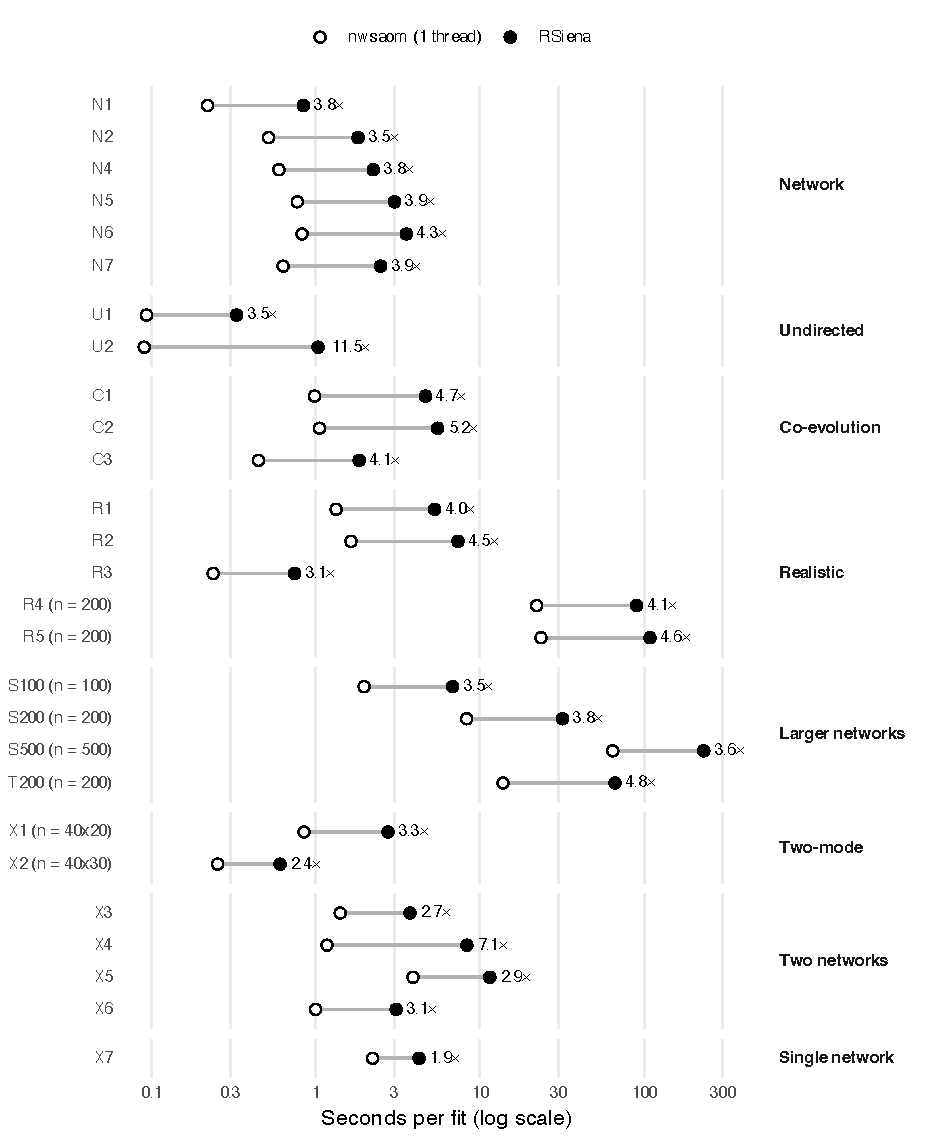
\includegraphics[width=\textwidth]{fig_bench_time.pdf}
\caption{Median seconds per fit of \nwsaom{} and RSiena for every model of the
benchmark, both on one thread.}
\end{figure}

\subsection{Several cores}

The comparison above is on one thread: RSiena's default, and \nwsaom{} with
\opt{cores(1)}. The table below gives \nwsaom{} with several threads against RSiena's
option for several processes (\texttt{useCluster = TRUE}); with several cores in
both programs, \nwsaom{} was \coresRfourvsrsbest{} to \coresRfivevsrsbest{} times as
fast as RSiena's best time. \nwsaom{}'s estimates are identical for every number of
threads.

\begin{table}[htbp]
\centering
\caption{\texttt{nwsaom} with 1 to 10 threads (in parentheses, speed-up over one thread) and RSiena with 1, 5 and 10 R processes: median seconds per fit over three seeds. The estimates of \texttt{nwsaom} are identical for every number of threads.}
\label{tab:cores}
\footnotesize
\begin{tabular}{lrrrrrrrr}
\toprule
 & & \multicolumn{4}{c}{\texttt{nwsaom}} & \multicolumn{3}{c}{RSiena, processes} \\
\cmidrule(lr){3-6}\cmidrule(lr){7-9}
Model & $n$ & \texttt{cores(1)} & \texttt{cores(2)} & \texttt{cores(5)} & \texttt{cores(10)} & 1 & 5 & 10 \\
\midrule
R1 & 50 & 1.34 (1.0) & 1.11 (1.2) & 0.96 (1.4) & 0.92 (1.5) & 4.74 & 3.53 & 3.97 \\
R4 & 200 & 22.0 (1.0) & 18.1 (1.2) & 15.4 (1.4) & 14.7 (1.5) & 89.5 & 34.4 & 29.7 \\
R5 & 200 & 23.6 (1.0) & 14.0 (1.7) & 11.7 (2.0) & 10.9 (2.2) & 111 & 46.0 & 49.1 \\
\bottomrule
\end{tabular}
\end{table}


\subsection{What was not measured}

RSiena's C++ code was not profiled internally, so the split of the remaining factor
among the design choices above is an inference from the source code. \nwsaom{}'s
Phase 2 counts are known to within 24 iterations per subphase. The timings come from
one machine that also ran other jobs; the one-minute load average was recorded
before every fit, at a median of 2.8 for the \nwsaom{} fits and 2.3 for RSiena's,
on 18 cores with single-threaded fits.
